
%Characterize the system, give all details that matter. Describe how the experimental procedure went.

% CAS codes Hinzufügen?

\subsection{Chemicals}
The following experiments were conducted using acetone (\qty{58.8}{\gram\per\mole}), from \texttt{Sigma Aldrich}, puriss. p.a., ($\geq$\qty{99.5}{\percent}), n-hexane (\qty{86.18}{\gram\per\mole}), from \texttt{Sigma Aldrich}, ($\geq$\qty{95}{\percent}) and methanol (\qty{32.04}{\gram\per\mole}), from \texttt{VWR Chemicals}, ($\geq$\qty{99.5}{\percent}). All chemicals were used forgoing any further purification.

\subsection{Procedure}
A total of 3 experiments were prepared and carried out as follows:

\subsubsection{Verification}

The identity and purity of acetone and n-hexane were verified by determining their respective \textit{refractive index} and \textit{density}. 

\textit{Refractive index} measurements were done via digital refractometer \texttt{ATAGO RX-5000} operating at standard wavelength of \qty{589.0}{\nano\meter} (D-line) and with samples maintained at a constant \qty{20.00 \pm 0.02}{\celsius} by a \texttt{LAUDA E100} circulation thermostat (attached to the refractometer). After ensuring the glass surface of the sample block was dry, a small amount of liquid was applied – just enough to cover the circular surface – and once equilibration was reached as indicated by the temperature display, measurements could be initiated.

\textit{Density} was determined in two different ways.

First, by \textit{method A}, filling a \qty{25.00 \pm 0.04}{\milli\liter} volumetric flask (insert marke) with either liquid and measuring its mass using a \texttt{METTLER-TOLEDO AG204 Delta Range} analytical balance, the accuracy range of which is stated as \qty{0.1}{\milli\gram} by the manufacturer.

And secondly, by \textit{method B}, using an \texttt{ANTON PAAR DMA 48} density gauge (Fig. \ref{fig:sketch_rho}), where the respective sample was carefully inserted via plastic syringe and – after visual confirmation that there were no air bubbles inside the u-shaped glass tube – run at setting \mintinline{R}{F505}. Between measurements of different samples, the tube was rinsed with deionized water and dried by inducing airflow.

\begin{figure}[H]
    \centering
    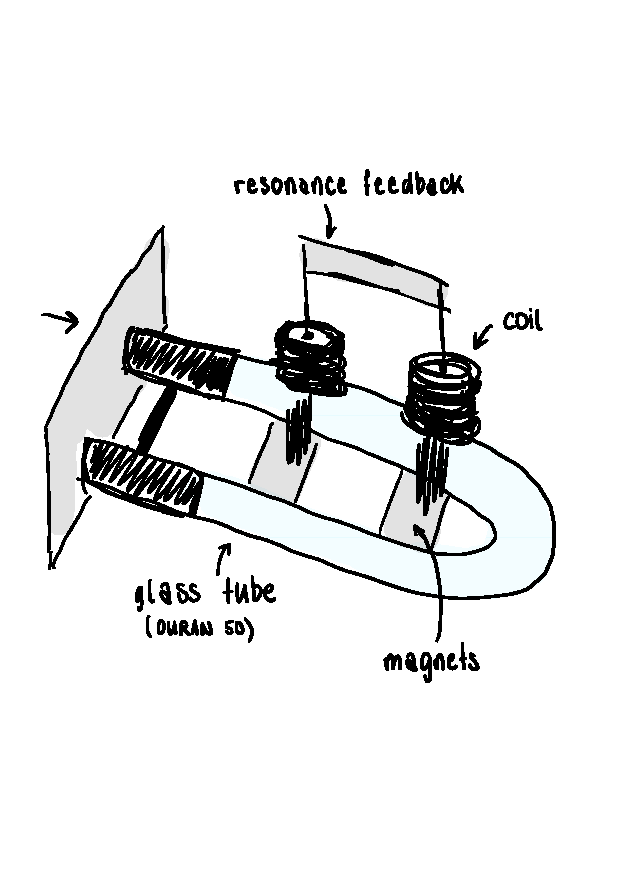
\includegraphics[width=.5\textwidth]{figures/sketch_density_meter.pdf}
    \caption{The \texttt{ANTON PAAR DMA 48} density gauge measures a liquid's density by oscillating a glass tube. The resonant frequency of the glass tube is directly correlated to the liquid's density.}
    \label{fig:sketch_rho}
\end{figure}


%\newpage

\subsubsection{Vapor Pressure}

\begin{figure}[H]
    \centering
    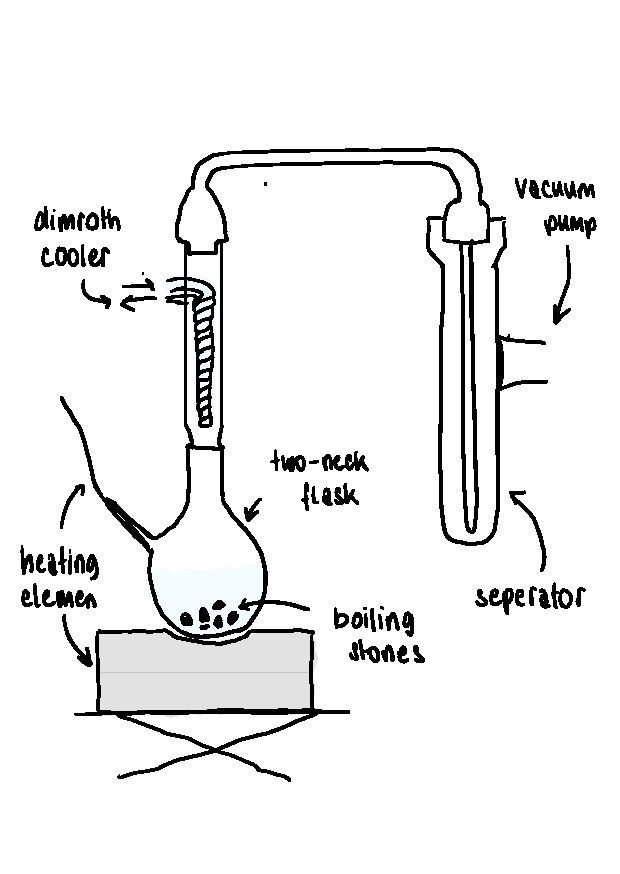
\includegraphics[width=.5\textwidth]{figures/ddr_sketch_setup.pdf}
    \caption{The vapor pressure measurement setup allows temperature and pressure to be controlled while observing the phase transition of the liquid.}
    \label{fig:sketch_setup}
\end{figure}

The boiling temperatures of acetone and n-hexane were measured at different pressure settings. 

For this purpose, a two necked flask containing the sample and about 10-15 boiling stones and filled to approximately half its capacity was attached to a pre-prepared setup (Fig.\ref{fig:sketch_setup}), omitting grinding grease due to the risk of contaminating the sample and comparatively low significance of a tight seal in this experiment.

Only after ensuring that all openings were closed, the \texttt{BÜCHI VAC V-503} vacuum pump, dimroth condensation cooler and \texttt{WINKLER WHLG2} laboratory heating mantle with a \texttt{WL10} heating controller were turned on. It is important to note that forgoing the former here and starting the cooler before sealing the system would allow water vapor from the air to condense inside the cooler and likely lead to falsified results. 

While maintaining a low heat supply via the controllable heating mantle, pressure within the system was steadily decreased under close surveillance through evacuation by means of a \texttt{BÜCHI I-100} vacuum controller and a ventilation valve until about \qty{150}{\milli\bar} and \qty{100}{\milli\bar} were reached for acetone and n-hexane respectively and the liquid was simultaneously boiling inside the flask and dripping steadily from the cooler. For acetone we could not observe any dripping at first, yet the liquid seemed to be boiling and the temperature was quickly decreasing to under \qty{10}{\celsius}. We concluded that the vapor currently forming would be at a lower temperature than the liquid in the dimroth cooler, causing it to escape into the separator instead of condensing. As such we increased our heat supply and not long after, equilibrium returned to the system and steady dripping could be observed. 

The temperature measured by the \texttt{GREISINGER GMH 3210} digital temperature gauge (with a resolution of \qty{0.1}{\kelvin}) was marked down with its corresponding vapor pressure and the pressure was incremented in \qtyrange{25}{50}{\mbar} steps until reaching \qty{900}{\mbar}, waiting for the temperature to level out after each increase and recording respective values. This was repeated at decreasing pressure, generating two sets of values for each sample.

%\newpage

\subsubsection{Evaporation Cooling}

\begin{figure}[H]
    \centering
    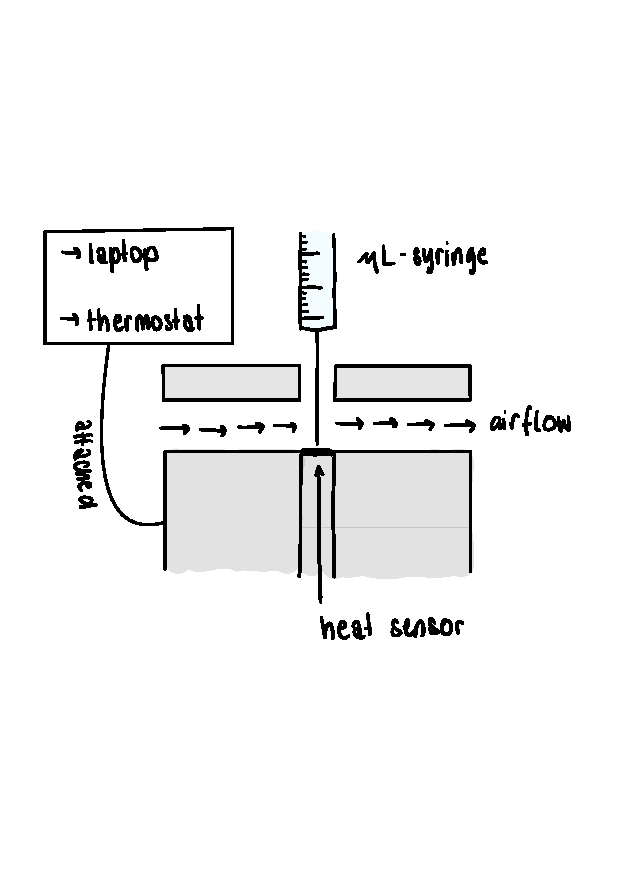
\includegraphics[width=.5\textwidth]{figures/ddr_sketch_TREVAC.pdf}
    \caption{The \texttt{TREVAC} evaporation cooling measurement system causes the liquid to evaporate and draw heat from the sensor plate, resulting in a temporary temperature drop.}
    \label{fig:sketch_trevac}
\end{figure}


The evaporation cooling effect of acetone, n-hexane and methanol (reference sample) were visualized and recorded by measuring the surface temperature of an ultra-sensitive heat sensor at \qty{0.25}{\second} intervals during the evaporation of a predefined volume of liquid sample applied to the sensor.

The setup, a \texttt{TREVAC}-apparatus (transient evaporation cooling) as can be seen in Fig. \ref{fig:sketch_trevac}, self-developed by the \texttt{PCL} at \texttt{ETH Zürich}, relies on a \texttt{LAUDA Ecoline 103} thermostat to keep the aluminium block with the \texttt{NATIONAL LM 35} heat sensor at its center at a programmable base temperature of 

$T_0=$ \qty{35}{\celsius}, 
\\deviating less than \qty{\pm 0.01}{\kelvin}. $T_0$ was selected at \qtyrange{30}{40}{\kelvin} below the boiling point of the lowest-boiling liquid. The sample was inserted at a steady pace via a \texttt{HAMILTON 801 RN} microliter syringe (scale facing forward to ensure measurement circumstances were as similar as possible for each sample inserted), using a measuring gauge to measure out exactly \qty{5}{\micro\liter} and discard any excess liquid beforehand. 

The registered surface temperature over time was recorded via analog/digital converter (ADC, 23 bit) and broadcast on the display of a laptop attached to the setup. 

This process was repeated 3 times per substance, leaving enough time for the sensor to equilibrate back to $T_0$ between the end of each prior evaporation and insertion of the current sample.
